\documentclass[14pt, conference]{IEEEtran}
\ifCLASSINFOpdf
\else
\fi

\IEEEoverridecommandlockouts

\usepackage{listings}
%\usepackage{xcolor}
\usepackage[table, svgnames]{xcolor}
\definecolor{codegreen}{rgb}{0,0.6,0}
\definecolor{codegray}{rgb}{0.5,0.5,0.5}
\definecolor{codepurple}{rgb}{0.58,0,0.82}
\definecolor{backcolour}{rgb}{0.5,1,0.5}
 
\lstdefinestyle{mystyle}{
    backgroundcolor=\color{backcolour},   
    commentstyle=\color{codegreen},
    keywordstyle=\color{magenta},
    numberstyle=\tiny\color{codegray},
    stringstyle=\color{codepurple},
    basicstyle=\footnotesize,
    breakatwhitespace=false,         
    breaklines=true,                 
    captionpos=b,                    
    keepspaces=true,                 
    numbers=none,                    
    numbersep=5pt,                  
    showspaces=false,                
    showstringspaces=false,
    showtabs=false,                  
    tabsize=2
}
 
\lstset{style=mystyle}


\usepackage{float}
\usepackage{longtable}
\usepackage{graphicx}
\usepackage{multirow}
%\usepackage{subcaption}
\usepackage{flushend}
%\usepackage{hyperref}
\usepackage{tabularx} 
\usepackage{booktabs} % For formal tables
\usepackage{hhline}
\usepackage{array}

\colorlet{headercolour}{DarkSeaGreen}
\AtBeginEnvironment{tabular}{\rowcolors{1}{\ifnumequal{\rownum}{1}{headercolour}{white}}{}}%

\newcolumntype{L}[1]{>{\raggedright\let\newline\\\arraybackslash\hspace{0pt}}m{#1}}
\newcolumntype{C}[1]{>{\centering\let\newline\\\arraybackslash\hspace{0pt}}m{#1}}
\newcolumntype{R}[1]{>{\raggedleft\let\newline\\\arraybackslash\hspace{0pt}}m{#1}}
\bibliographystyle{IEEEtran}

\usepackage{cite}
% \usepackage{amsmath,amssymb,amsfonts}
\usepackage{algorithmic}
\usepackage{graphicx}
\usepackage{textcomp}
\def\BibTeX{{\rm B\kern-.05em{\sc i\kern-.025em b}\kern-.08em
    T\kern-.1667em\lower.7ex\hbox{E}\kern-.125emX}}

%\hypersetup{bookmarks=false}

\begin{document}

\title{Network Anomaly Detection Using LightGBM: \\ A Gradient Boosting Classifier}

\author{
\IEEEauthorblockN{Md. Khairul Islam\textsuperscript{1},
Prithula Hridi\textsuperscript{1}, Md. Shohrab Hossain\textsuperscript{1}, Husnu S. Narman\textsuperscript{2}}

\IEEEauthorblockA{\textsuperscript{1}Department of Computer Science and Engineering, Bangladesh University of Engineering and Technology, Bangladesh\\
    \textsuperscript{2}Weisberg Division of Computer Science, Marshall University, Huntington, WV, USA\\}
\IEEEauthorblockA{Email:  khairulislamtanim@gmail.com, prithula5117@gmail.com, mshohrabhossain@cse.buet.ac.bd,  narman@marshall.edu}
}

\maketitle

\begin{abstract}
Anomaly detection systems are significant in recognizing intruders or suspicious activities by detecting unseen and unknown attacks. In this paper, we have worked on a benchmark network anomaly detection dataset UNSW-NB15, that reflects modern-day network traffic. Previous works on this dataset either lacked a proper validation approach or followed only one evaluation setup which made it difficult to compare their contributions with others using the same dataset, but with different validation steps. In this paper, we have used a machine learning classifier LightGBM to perform binary classification on this dataset. We have presented a thorough study of the dataset with feature engineering, preprocessing, feature selection. We have evaluated the performance of our model using different experimental setups (used in several previous works)  to clearly evaluate and compare with others. Using ten-fold cross-validation on the train, test, and combined (training and test) dataset, our model has achieved 97.21\%, 98.33\%, and 96.21\% f1\_scores, respectively. Also, the model fitted only on train data, achieved 92.96\% f1\_score on the separate test data. So our model also provides significant performance on unseen data. We have presented complete comparisons with the prior arts using all performance metrics available on them. And we have also shown that our model outperformed them in most metrics and thus can detect network anomalies better.

\end{abstract}

\begin{IEEEkeywords}
anomaly detection, machine learning,  network security.
\end{IEEEkeywords}
%------------------------ Into \input{introduction.tex}

\section{Introduction}
Web applications are getting increasingly popular, and the Internet has become an important part in our day-to-day life. As a
consequence, network systems are being targeted more by attackers with malicious intent. To detect intruders in a
network system, there are generally two approaches: signature-based and anomaly-based detection. Signature-based systems maintain a database of previously known attacks and raise alarms when any match is found with the analyzed data. However, they are vulnerable to zero-day attacks.

An anomaly in a network means a deviation of traffic data from its normal pattern. Thus, anomaly detection techniques have the advantage of detecting zero-day attacks. However, in a complex and large network system,  it is not easy to define a set of valid requests or normal behavior of the endpoints. Hence, anomaly detection faces the disadvantage of having a high false-positive error rate (events erroneously classified as attacks). There are different types of anomalies that can be mapped with different types of attacks. According to Ahmed et al.\cite{ahmed2016survey}, the main attack types are DoS, Probe, User to Root (U2R), and Remote to User (R2U) attacks. Ahmed et al. \cite{ahmed2016survey} mapped the point anomaly with the U2R and the R2U attacks, the DoS attack to the collective anomaly, and the Probe attack to the contextual anomaly.

With the advance of machine learning and deep learning techniques, in many cases they have outperformed the previous state-of-the-art models. As UNSW-NB15 \cite{moustafa2015unsw} is a benchmark network anomaly detection dataset, numerous studies have been done on it.
However, to evaluate the same dataset different setups were adopted (Section \ref{relatedWorks}). For example, train and evaluate on train data \cite{mogal2017nids, Kanimozhi2019UNSW-NB15} . Ten-fold cross validation on train data \cite{suleiman2018performance, meftah2019network}), test data \cite{hanif2019intrusion}, combined (train+test) data  \cite{nawir2019effective, koroniotis2017towards}. Five-fold cross validation on train and test data \cite{meghdouri2018analysis} . Train on train data and evaluate on test data  \cite{bhamare2016feasibility, moustafa2016evaluation}.


% \begin{itemize}
%     \item Train and evaluate on train data (Mogal et al. \cite{mogal2017nids}, Kanimozhi et al. \cite{Kanimozhi2019UNSW-NB15} )
%     \item Ten-fold cross validation on 
%         \begin{itemize}
%             \item Train data (Suleiman et al. \cite{suleiman2018performance}, Meftah et al. \cite{meftah2019network})
%             \item Test data (Hanif et al. \cite{hanif2019intrusion})
%             \item Combined (test + train) data (Nawir et al. \cite{nawir2019effective}, Koroniotis et al. \cite{koroniotis2017towards})
%         \end{itemize}
%     \item Five-fold cross validation on train and test data (Meghdouri et al. \cite{meghdouri2018analysis})
%     \item Train on train data and evaluate on test data (Bhamare et al. \cite{bhamare2016feasibility}, Moustafa et al. \cite{moustafa2016evaluation})
% \end{itemize}

With so many different experimental setups, it is difficult to find the single best work on this dataset. Moreover, works that followed the same experimentation setup did not compare their results with prior works in some cases (for example, Kanimozhi et al. \cite{Kanimozhi2019UNSW-NB15} and Nawir et al. \cite{nawir2019effective} did not compare their results with  Koroniotis et al. \cite{koroniotis2017towards}). Therefore, it is difficult to validate their improvements. Mogal et al. \cite{mogal2017nids} and Kanimozhi et al. \cite{Kanimozhi2019UNSW-NB15} mentioned near-perfect detection scores. However, they did not mention the significant technical flaws regarding their approaches, which we have explained in Section \ref{sec:validationOnSame}.  Some other works \cite{nawir2019effective, Kanimozhi2019UNSW-NB15, meghdouri2018analysis} followed only one validation setup. Hence, it is impossible to compare those works with the ones, which have worked on the same dataset but with different validation setups.

The novelty and contributions of this work are as follows:
\begin{itemize}
    \item We have provided a thorough study of the UNSW-NB15 dataset with feature engineering, preprocessing, selection. Previous studies did not use feature engineering to improve results.
    \item We have explored the performance of a boosting algorithm in binary classification on the dataset following all experimentation setups found from prior studies whereas each of the previous works focused on only one setup.
    \item We have compared our results to prior state-of-the-art works using all related performance metrics.
\end{itemize}

% Brief summary of major findings of results
Our results show that feature engineering can make the model more generalized. So our model performance improved in cross-validation experiments, as well as when evaluated on separate test data. We have also shown a very small false alarm rate (1.83\% - 4.81\%), so the common weakness of using anomaly detection techniques would not happen for our model. 
%Application of this work
Our work can help in detecting unseen anomaly attacks better having very few false alarms. And Our different experimentation setups will help visualize the impact of validation strategies on the model performance of this dataset.


The rest of the paper has been organized as follows. Section\ref{relatedWorks} describes the recent works related to NIDS (Network Intrusion Detection Systems) on the UNSW-NB15 dataset. Our proposed methodology has been explained in
Section \ref{methodology}. Section \ref{results} describes the experimentation setups and our results as well as some comparisons with the prior state-of-the-art. 
The rest of the comparisons regarding evaluating on train and test data, cross-validation approaches have been shown in Section
\ref{comparison}. Finally, Section\ref{conclusion} has the concluding remarks.


%---- Related works ------------------------
%---- Related works ------------------------
%---- Related works ------------------------

\section{Related works} 
\label{relatedWorks}

For network intrusion detection KDDCUP99, NSL-KDD, DARPA, UNSW-NB15 are among the benchmark dataset. As a popular dataset, we focus on binary classification of the UNSW-NB15 dataset \cite{moustafa2015unsw}  which is used in several anomaly detection works. Based on the model evaluation process, we have divided them into several parts.

\subsection{Random train test}
Moustafa et al. \cite{moustafa2017hybrid} used central points of attribute values and Association Rule Mining for feature
selection on a high level of abstraction from datasets UNSW-NB15 and NSL-KDD. They have partitioned the datasets into train and test sets following an equation. Then evaluated performance using Expectation-Maximisation clustering (EM), Logistic Regression (LR), and Naïve Bayes (NB). 
%The LR produced the best results on the two datasets with accuracy and FAR, 83\% and 14.2\% on the UNSW-NB15 dataset, 82.1\% and 17.5\% on the NSL-KDD dataset. 
Moustafa et al. \cite{moustafa2018anomaly} also proposed a beta mixture model-based anomaly detection system on the UNSW-NB15 dataset. They first selected eight features from the dataset,
then randomly selected samples from it. 
% The best result had accuracy 93.4\%, detection rate 92.7\%, and a false-positive rate 5.9\%. 
In another work, Moustafa et al. \cite{moustafa2019holistic} selected random samples from the UNSW-NB15 dataset and ran ten-fold cross-validation on it. % They found the LogisticRegression classifier to achieve the best result with 95.6\% accuracy and a 5.6\% false alarm rate.

\subsection{Validation on same data used for training}
Mogal et al.\cite{mogal2017nids} used machine learning classifiers on both UNSW-NB15 and KDDCUP99 datasets.
They achieved nearly 100\% accuracy on both datasets using Naive Bayes and Logistic Regression on train data. Kanimozhi et al. \cite{Kanimozhi2019UNSW-NB15} choose the best four features of
the UNSW-NB15 dataset using the RandomForest classifier. They also used a Multi-Layer Perceptron to show how neural
networks would perform on this dataset. 

\subsection{Cross validation}
Koroniotis et al.\cite{koroniotis2017towards} selected the top ten features of the UNSW-NB15 combined (train+test)
dataset using Information Gain Ranking Filter. Then they ran ten-fold cross-validations using machine learning techniques.
Among the techniques applied, DT (Decision Tree C4.5 Classifier) performed the best at distinguishing between Botnet and normal network traffic.
 
 Suleiman et al. \cite{suleiman2018performance} explored the performance of machine learning classifiers on benchmark
and new datasets (UNSW-NB15, NSL-KDD, and Phishing) using ten-fold cross-validation. They found the RandomForest
classifier to perform the best. All the experiments were done using the WEKA tool. 
Nawir et al. \cite{nawir2019effective} applied ten-fold cross-validation on the binary classification of the combined
(train+test) dataset by using the WEKA tool. They also compared centralized and distributed AODE algorithms based on accuracy against the number of nodes. 

Meftah et al. \cite{meftah2019network} applied both binary and multiclass classification on the UNSW-NB15 dataset. They found for binary classification SVM performs the best in ten-fold
cross-validation and decision tree (C5.0) for multiclass classification.
% with 82.11\% accuracy and decision tree (C5.0) perform the best for multiclass classification with 86\% f-measure and 85.41\% accuracy on train data. 
Hanif et al. \cite{hanif2019intrusion} used ANN(Artificial Neural Network) on the same dataset. The neural network had one hidden layer and it achieved an average 84\% accuracy and less
than 8\% false-positive rate in repeated cross-validation. They compared their performance with prior works on the NSL-KDD dataset, instead of works on the same dataset. Meghdouri et al. \cite{meghdouri2018analysis} applied feature preprocessing and principal component analysis on the UNSW-NB15 dataset. Then performed five-fold cross-validation using a RandomForest classifier.
 % and achieved 84.9\% f-measure.

\subsection{Validation on separate test data}
Moustafa et al. \cite{moustafa2016evaluation} analyzed the statistical properties of the UNSW-NB15 dataset. The complexity of the dataset was evaluated using five techniques (DT, LR, NB, ANN, and EM clustering). There, based on the performance results UNSW-NB15 was found to be more complex compared to the KDD99 dataset. Vinaykumar et al. \cite{vinayakumar2019deep} used classical machine learning classifiers, and deep neural networks on several intrusion detection datasets. The classical models performed much better than the neural network models.
Dahiya et al. \cite{dahiya2018network} applied feature reduction techniques on both larger and smaller versions of the UNSW-NB15 dataset. Bhamare et al. \cite{bhamare2016feasibility} tested the robustness of machine learning models in cloud scenarios. They trained classifiers on the UNSW-NB15 dataset and tested them on a cloud security dataset ISOT. Bhamare et al. \cite{bhamare2016feasibility} found that these models did not perform well in cloud environment.

\subsection{Others}
Viet et al. \cite{viet2018using} used a deep learning model on the UNSW-NB15 and NSL-KDD datasets only to detect network scanning attacks. In UNSW-NB15 as the scanning types are
labeled altogether, so they applied binary classification for it.

% Using the Deep Belief Network, they achieved TPR and FAR, 99.86\% and 2.76\%  on the UNSW-NB15 dataset, 99.458\% and 2.71\% on the NSL-KDD dataset.
% Moustafa et al. \cite{moustafa2015significant} studied the significant features of the UNSW-NB15 and KDD99 dataset. The results show the original KDD99 attributes are less efficient than the replicated UNSW-NB15 attributes of the KDD99 data set.  
% Belouch et al. \cite{belouch2018performance} used machine learning classifiers to detect network intrusions on the UNSW-NB15 dataset on Apache Spark. 
% Their RandomForest classifier achieved 97.49\% accuracy on the train dataset. 

\subsection{Gap analysis}
To the best of our knowledge, there has been no work that has provided a thorough study of the UNSW-NB15 dataset with feature engineering to improve results. Moreover, most of the previous works on this dataset focused on only one evaluation process. So it is difficult to make a proper comparison among them. For example, the performance achieved in five-fold cross-validation, can not be compared with that achieved in ten-fold cross-validation. So, we have evaluated our model performance using all possible experimentation setups found in prior arts and provided a thorough comparison with prior state-of-the-art techniques. We have also used feature engineering to reduce overfitting, thereby providing a more generalized model.


%--------------------------------------------

\section{Proposed Methodology} \label{methodology}
We have targeted only to perform binary classification on the dataset. We have used Kaggle kernels for running our models. It provided us with 4 CPU cores, 16 Gigabytes of RAM when this work was done. In the following subsections,  we have described how the dataset was prepared for experimentation and the performance metrics used for evaluation. 


\subsection{Dataset Description}
We have used the UNSW-NB15 dataset\cite{moustafa2015unsw} which is a recent benchmark dataset for NIDS (Network Intrusion Detection Systems). The dataset was created at the Cyber Range Lab of the Australian Center of Cyber Security. Compared to other existing datasets (such as KDDCup99, NSL-KDD, DARPA), the UNSW-NB15 dataset is more recent and better reflects modern network traffic. UNSW-NB15 represents nine major families of attacks by utilizing the IXIA PerfectStorm tool. The main data set contains 2,540,044 observations. The authors divided a part of this data set was divided into train and test sets, which has been used in this work. The dataset description is shown in Table \ref{datasetDescription}. We have considered binary classification for this study. Hence, we have only predicted whether the record is attack type or normal. The dataset labels class 0 for normal and 1 for attack records. From Table \ref{datasetDescription} we can see the train data is imbalanced. The majority of the records are anomalies. However, in the test data, they are nearly balanced. 



\begin{table}
\normalsize
\centering
\caption{UNSW-NB15 Dataset Description}
\label{datasetDescription}
\renewcommand{\arraystretch}{1.2}

\begin{tabular}{|C{3cm}|C{2cm}|C{2cm}|}
\hline
 \textbf{Type} & \textbf{Train} & \textbf{Test} \\ \hline
Normal & 56,000 & 37,000 \\ \hline
Anomaly & 119,341 & 45,332 \\ \hline
\textbf{Total}  & \textbf{175,341} & \textbf{82,332} \\ \hline
\end{tabular}
\end{table}

In the following list, we have described the features provided by the larger UNSW-NB15 dataset. 

\begin{itemize}
\item  id:Record id no.
\item proto : Transaction protocol.
\item state:Indicates to the state and its dependent protocol, for example : ACC, CLO, CON.
\item dur :Record total duration.
\item sbytes:Source to destination transaction bytes.
\item dbytes:Destination to source transaction bytes.
\item sttl: Live value of source to destination time.
\item dttl:Live value of destination to source time.
\item sloss:Source packets retransmitted or dropped.
\item dloss:Destination packets retransmitted or dropped.
\item service: http, ftp, smtp, ssh, dns, ftp-data ,irc  and (-) if not much used service.
\item sload:Source bits per second.
\item dload:Destination bits per second.
\item spkts:Source to destination packet count.
\item dpkts:Destination to source packet count.
\item swin:Source TCP window advertisement value.
\item dwin:Destination TCP window advertisement value.
\item stcpb:Source TCP base sequence number.
\item dtcpb:Destination TCP base sequence number.
\item smean:Mean of the packet size transmitted by the source.
\item dmean:Mean of the packet size transmitted by the destination.
\item trans\_depth: The pipelined depth into the connection of http request/response transaction.
\item response\_body\_len: The actual uncompressed content size of the data transferred from the server’s http service.
\item sjit: Source jitter (mSec).
\item djit: Destination jitter (mSec).
\item rate: a feature based on record start and end time.
\item sinpkt: Source interpacket arrival time (mSec).
\item dinpkt: Destination interpacket arrival time (mSec).
\item tcprtt: TCP connection setup round-trip time. The sum of ’synack’ and ’ackdat’.
\item synack: TCP connection setup time. The time between the SYN and the SYN\_ACK packets.
\item ackdat: TCP connection setup time. The time between the SYN\_ACK and the ACK packets.
\item is\_sm\_ips\_ports: If source and destination IP addresses are equal and port numbers equal then, this variable takes value 1 else 0.
\item is\_ftp\_login:If the ftp session is accessed by user and password then 1 else 0.

\end{itemize}

The following features are calculated in the last 100 connections from the current record.
\begin{itemize} 
% \setcounter{enumi}{33}
\item ct\_state\_ttl: According to specific range of values of source/destination time to live for each stat .
\item ct\_flw\_http\_mthd :Number of flows that has  Get and Post methods in http service.

\item ct\_ftp\_cmd: Number of flows that has a command in ftp session.
\item ct\_srv\_src: Number of connections that contain the same address for service and source.
\item ct\_srv\_dst: Number of connections that contain the same address for service  and destination.
\item ct\_dst\_ltm: Number of connections of the same destination address.
\item ct\_src\_ltm:Number of connections of the same source address.
\item ct\_src\_dport\_ltm:Number of connections of the same source address and the destination port.
\item ct\_dst\_sport\_ltm:Number of connections of the same destination address and the source port.
\item ct\_dst\_src\_ltm: Number of connections of the same source and the destination address.
\end{itemize}

There are two labeled target columns :
\begin{itemize} 
% setcounter{enumi}{43}
    \item attack\_cat: The name of each attack category. They are Fuzzers, Analysis, Backdoors, DoS Exploits, Generic, Reconnaissance, Shellcode, and Worm.
 \item Label:0 for normal and 1 for attack records.
\end{itemize}

\subsection{Preprocessing \label{preprocessing}}
We have performed the preprocessing on the data set using the following steps :

\subsubsection{Dropping unnecessary columns}
We have dropped the id column as it can not be learned as a feature. Also, we have dropped the attack\_cat, which is the category of the anomaly type. And the label column is our target. So among 45 columns, 42 were used in the feature set.

\subsubsection{Feature engineer categorical columns}
We have found many categorical labels to have a very low frequency. To make it easier for the model to learn from these categorical features, labels with low frequency were converted into a single label.

\begin{itemize}
    \item For state features, except the top five labels by frequency ('FIN', 'INT', 'CON', 'REQ', 'RST') other labels were converted into label 'others'.
    \item For service columns, labels except '-', 'dns', 'http', 'smtp', 'ftp-data', 'ftp', 'ssh', 'pop3' were converted into 'others' labels. 
    \item For the proto column, 'igmp', 'icmp', 'rtp' labels were combined into the label 'igmp\_icmp\_rtp'. Then labels except 'tcp', 'udp', 'arp', 'ospf', 'igmp\_icmp\_rtp' were converted into label 'others'. 
\end{itemize}

Before this, test data had new categorical values present. However, after this feature engineering, categorical value sets for train and test data became the same. That enabled us to use one-hot encoding on the dataset. If any categorical value present in test data was never present in train data. Then in one-hot encoding, there will be no column for it in the train, but it will in test data. So the column mismatch will make the prediction difficult. 


\subsubsection{Scaling}
We have applied StandardScaler from sklearn's preprocessing library on all non-categorical features. It was fitted on the train data, then the fitted scaler was used to convert both train and test data. It converts values using the following equation:
\begin{equation}
    x = \frac{x-\mu}{\sigma}
\end{equation}

where $\mu$ is the mean value and $\sigma$ is the standard deviation.

\subsubsection{Feature Selection}
We have used the RandomForest classifier of sklearn with default parameters to calculate feature importance on the
train dataset. We have first preprocessed the dataset using previous steps. Then averaged feature importance over ten-fold
cross-validation. We have converted the values into percentages, for easier understanding. Then sorted them in descending order.
From there we have chosen to drop features with less than 0.5\% importance value. The dropped 7 features are response\_body\_len,
spkts, ct\_flw\_http\_mthd, trans\_depth, dwin, ct\_ftp\_cmd, is\_ftp\_login. In Table \ref{featureImportance} we have shown the chosen features with corresponding importance.


\begin{table}
\normalsize
\centering
\caption{Feature Importance}
\label{featureImportance}
% increases cell padding
\renewcommand{\arraystretch}{1.2}
\begin{tabular}{|C{2.1cm}|C{1.1cm}|C{2.5cm}|C{1.1cm}|}
\hline
\textbf{Feature} & \textbf{Importance} & \textbf{Feature} & \textbf{Importance}\\ \hline

sttl & 16.53& sjit & 1.7  \\ \hline
ct\_state\_ttl & 11.06& dloss & 1.22  \\ \hline
dload & 7.2& proto & 1.21  \\ \hline
dttl & 4.93& djit & 1.14  \\ \hline
dmean & 4.19& sloss & 0.9  \\ \hline
ackdat & 3.8& ct\_src\_ltm & 0.83  \\ \hline
rate & 3.79& ct\_dst\_ltm & 0.83  \\ \hline
dinpkt & 3.51& stcpb & 0.81  \\ \hline
sbytes & 3.23& ct\_dst\_sport\_ltm & 0.8  \\ \hline
smean & 2.85& dtcpb & 0.75  \\ \hline
sload & 2.72& swin & 0.62  \\ \hline
state & 2.71& is\_sm\_ips\_ports & 0.57  \\ \hline
dpkts & 2.59& ct\_src\_dport\_ltm & 0.57  \\ \hline
tcprtt & 2.49& service & 0.51  \\ \hline
ct\_srv\_dst & 2.49& spkts & 0.47  \\ \hline
ct\_dst\_src\_ltm & 2.43& ct\_flw\_http\_mthd & 0.17  \\ \hline
sinpkt & 2.41& response\_body\_len & 0.16  \\ \hline
ct\_srv\_src & 2.2& trans\_depth & 0.14  \\ \hline
dbytes & 1.93& dwin & 0.02  \\ \hline
synack & 1.76& ct\_ftp\_cmd & 0.01  \\ \hline
dur & 1.76& is\_ftp\_login & 0.01  \\ \hline

\end{tabular}
\end{table}


\subsubsection{OneHotEncoding}
We have used pandas library to OneHotEncode all the categorical features. It became possible as after using feature engineering, categorical value sets became the same in train and test datasets. The final number of features in our dataset is 53.


\subsection{Evaluation metrics}
In this section, we have discussed the performance metrics we have used in our experiments on the UNSW-NB15 dataset \cite{moustafa2015unsw}. We have also used them to compare the performance of our approach with previous works.
%All the metrics were calculated using the sklearn.metrics module.

\begin{itemize}
    \item \textbf{True Positives (TP)}: The cases in which YES was predicted and the actual output was also YES.
    \item \textbf{True Negatives (TN}: The cases in which NO was predicted and the actual output was NO.
    \item \textbf{False Positives (FP)}: The cases in which YES was predicted and the actual output was NO.
    \item \textbf{False Negatives (FN)}: The cases in which NO was predicted and the actual output was YES.
\end{itemize}

\subsubsection{Accuracy}
It is the ratio of the number of correct predictions to the total number of input samples.
\begin{equation}
    Accuracy = \frac{TP+TN}{TP+TN+FP+FN}
\end{equation}

\subsubsection{Precision}
It is the ratio of the number of correct positive results to the number of positive results predicted by the classifier.
\begin{equation}
    Precision = \frac{TP}{TP+FP}
\end{equation}

\subsubsection{Recall or Detection Rate or True Positive Rate)}
It is the ratio of the number of correct positive results to the number of all relevant samples (all samples that should
have been identified as positive).
\begin{equation}
    recall = \frac{TP}{TP+FN}
\end{equation}

\subsubsection{F1\_score}
The harmonic means of precision and recall.
\begin{equation}
    f1\_score = 2 * \frac{1}{\frac{1}{precision}+ \frac{1}{recall}}
\end{equation}

\subsubsection{False Positive Rate (FPR)}
It is the proportion of incorrectly identified observations.
\begin{equation}
    FPR = \frac{FP}{FP+TN}
\end{equation}

\subsubsection{False Alarm Rate (FAR)}
The probability that a record gets incorrectly classified.
\begin{equation}
    FAR = \frac{FP+FN}{FP+FN+TP+TN}
\end{equation}

\subsubsection{ROC AUC}
It computes the Area Under the Receiver Operating Characteristic Curve (ROC AUC) from prediction scores.


% \subsubsection{Time (sec)}
% As run time is an important factor in detecting network anomalies, we have determined the time required to run our models. 
%We have used the time library of python for this purpose.


\section{Experiment and Results \label{results}}
For evaluating the UNSW-NB15 dataset, we have performed ten-fold cross-validation using Stratified KFold of the sklearn library with a random shuffle set to true. We have used several popular machine learning classifiers to measure the prediction performance. The models were run mostly with default parameters. We have set the random state to 1 for all of them so that the results are reproducible. All models except LightGBM \cite{ke2017lightgbm}, were from sklearn library version 0.23.0. During prediction, for LightGBM we used the best iteration. The used models are listed below with their important parameters.
\begin{enumerate}
    \item LogisticRegression : penalty = l2, max\_iter = 100, solver = lbfgs, C = 1.0
    \item GradientBoosting: learning\_rate = 0.1, n\_estimators = 100,max\_depth = 3
    \item DecisionTree: criterion = 'gini', max\_depth = None, max\_features = None,
    \item RandomForest: n\_estimators = 100, criterion = 'gini', max\_depth = None, max\_features = None
    \item LightGBM: learning rate = 0.1, objective = binary, metric = binary\_logloss,boost\_from\_average = True,
    num\_round = 2000, early\_stopping\_rounds = 50.
\end{enumerate}

The result of this experiment is shown in Table \ref{crossvalidationWithDifferentModels}. We have chosen the best model based on f1-score and accuracy. Here class labels are 0 for normal and 1 for attack records. So these metrics are the best choices to validate the model performance. As shown in Table \ref{crossvalidationWithDifferentModels}, LightGBM achieved the best performance in both accuracy (96.18\%) and f1-score (91.21\%). LightGBM ( Ke et al. \cite{ke2017lightgbm})is a highly efficient gradient boosting framework that uses tree-based learning algorithms. It follows a more complex leaf-wise split approach rather than a level-wise approach. Which reduces overfitting and improves the validation results. 

\subsection{Handling class imbalance}
From Table \ref{datasetDescription} we can see the train dataset is slightly imbalanced. The ratio of normal and anomaly records is 56: 119.  We used is\_unbalance and scale\_pos\_weight  parameters provided by LightGBM to test whether handling class imbalance will improve results. If is\_unbalance is set to true, LightGBM will automatically try to balance the weight of the dominated label. Using scale\_pos\_weight, we can manually set weight for the positive class. % However, the LightGBM official documentation \footnote{https://lightgbm.readthedocs.io/en/latest/Parameters.html} warns, using this should increase the overall performance metric of the model, but it will also result in poor estimates of the individual class probabilities. 
During ten-fold cross-validation in our experimentation, we found using these parameters decreases the f1\_score. So we have not used them finally. However, during predicting on separate test data, we have found setting is\_unbalance to true improves the prediction performance slightly.

\begin{table}
\normalsize
\centering
\caption{Ten-fold cross validation with different models}
\label{crossvalidationWithDifferentModels}
\renewcommand{\arraystretch}{1.2}

\begin{tabular}{|C{2.8cm}|C{2.1cm}|C{2.1cm}|}
\hline
\textbf{Metrics(\%)} & \textbf{Accuracy(\%)} & \textbf{F1\_score(\%)} \\ \hline
LogisticRegression & 93.54 & 95.42 \\ \hline
GradientBoosting & 94.58 & 96.11\\ \hline
DecisionTree  & 94.99 & 96.32\\ \hline
RandomForest  & 96.08 & 97.14 \\ \hline
LighGBM & 96.18 & 97.21 \\ \hline
\end{tabular}
\end{table}


\subsection{Validation on same data used for training}
\label{sec:validationOnSame}

Mogal et al. \cite{mogal2017nids}, Kanimozhi et al. \cite{Kanimozhi2019UNSW-NB15} evaluated model performance on the UNBSW-NB15 dataset without using any cross-validation approach. The same data used for training the model was used for validation too. To compare our model's performance with them, we have followed a similar setup. As evident from the results shown in Table \ref{evaluationOnTrainData}, this experimentation setup does not truly reflect model performance. As the model overfits on train data, its performance will be very poor on a separate test set. For example, we have found our model when overfitted on train data, only achieved 86.88\% accuracy and 89.14\% f1\_score on test data. So the models proposed by both of those prior works should not be used in reality.

\begin{table}
\normalsize
\centering
\caption{Evaluating model on data used for training}
\label{evaluationOnTrainData}
\renewcommand{\arraystretch}{1.2}

\begin{tabular}{|C{3.5cm}|C{1.8cm}|C{1.8cm}|}
\hline
\textbf{Metrics(\%)} & \textbf{Train} & \textbf{Test} \\ \hline
Accuracy & 99.60 & 99.98 \\ \hline
Precision & 99.52 & 99.97\\ \hline
Recall  & 99.89 & 99.98\\ \hline
F1\_score  & 99.71 & 99.98 \\ \hline
FPR & 0.01 & 0.0004\\ \hline
AUC & 99.99 & 99.99\\ \hline
Time(s) & 243 & 237\\ \hline
\end{tabular}
\end{table}


\subsection{Ten-fold cross validation}
Ten-fold cross-validation on train, test or combined(train+test) dataset was performed by Meftah et al. \cite{meftah2019network}, Suleiman et al. \cite{suleiman2018performance}, Nawir et al. \cite{nawir2019effective}, Hanif et al. \cite{hanif2019intrusion} . We have used the StratifiedKFold method of sklearn.model\_selection module with shuffle enabled to perform the ten-fold cross-validation. Average scores achieved in that process are shown in Table \ref{tenFoldCrossValidation}. The roc-auc curve for these three cases is shown in Figure \ref{fig:tenFold}. Interestingly we see cross-validation on test data has the best results. This can be because the test data is more balanced. 

\begin{table}
% this increases the fontsize used in table
\normalsize
\centering
\caption{Ten-fold cross validation}
\label{tenFoldCrossValidation}
% increases cell padding
\renewcommand{\arraystretch}{1.2}
\begin{tabular}{|C{2.3cm}|C{1.3cm}|C{1.3cm}|C{1.8cm}|}
\hline
\textbf{Metrics(\%)} & \textbf{Train} & \textbf{Test} & \textbf{Combined}\\ \hline
Accuracy & 96.18 & 98.18 & 95.19 \\ \hline
Precision & 96.54 & 98.87& 96.84\\ \hline
Recall  & 97.89 & 97.80 & 95.58\\ \hline
F1\_score  & 97.21 & 98.33 & 96.21\\ \hline
FPR & 7.47 & 1.37 & 5.51\\ \hline
FAR & 3.82 & 1.83 & 4.81 \\ \hline
AUC & 99.44 & 99.81 & 99.26\\ \hline
Time(s) & 628.1 & 281.1 & 838.8\\ \hline
\end{tabular}
\end{table}


\begin{figure}[!tbh]
\centering
  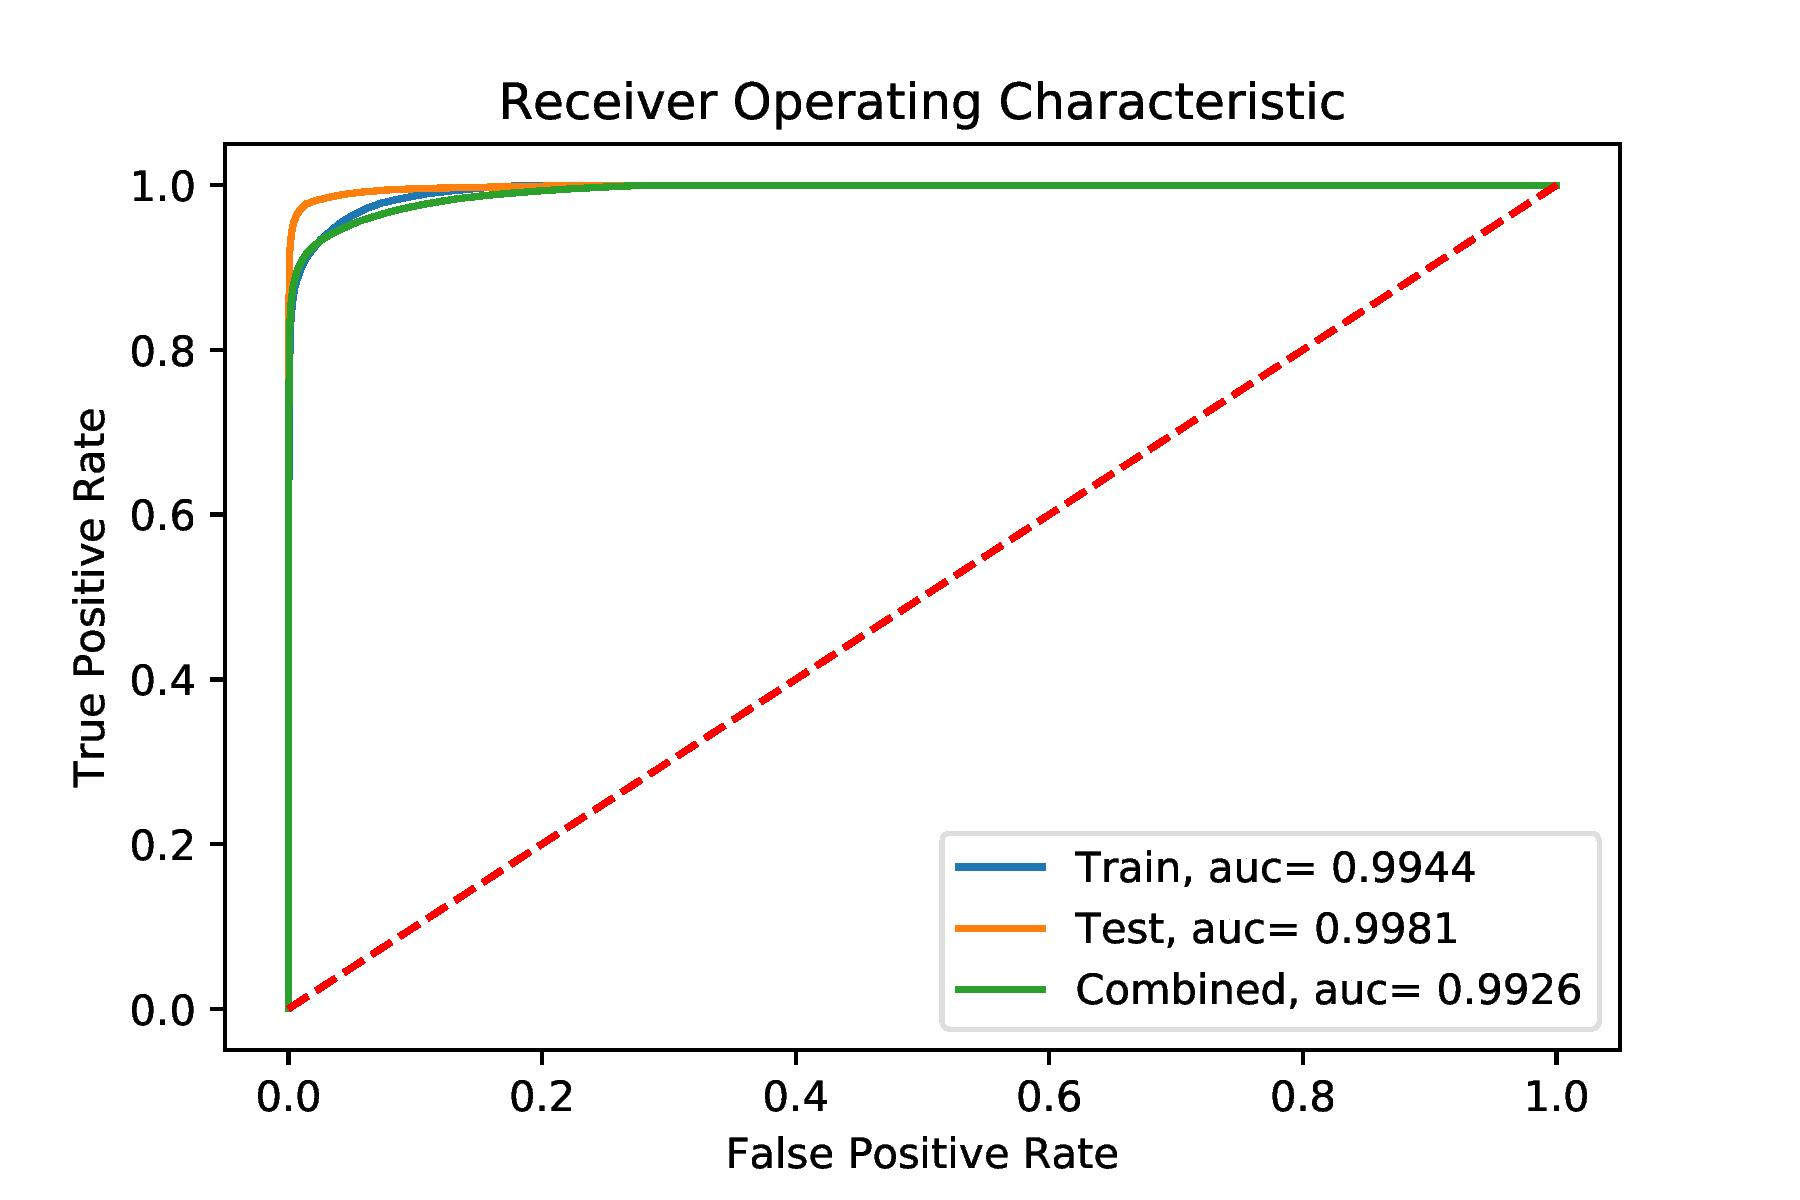
\includegraphics[width=\linewidth]{images/roc_ten.jpg}
  \caption{ROC-AUC curve for ten-fold cross validation}
\label{fig:tenFold}
\end{figure}


\subsection{Validation on test data \label{validationResultsOnTest}}
In this experiment we have validated the model trained on train data using the separate test dataset of UNSW-NB15 following Moustafa et al. \cite{moustafa2016evaluation}, Bhamare et al. \cite{bhamare2016feasibility}, Vinayakumar et al. \cite{vinayakumar2019deep}, Dahiya et al. \cite{dahiya2018network}. As  Meftah et al. \cite{meftah2019network}
mentioned, some columns have new labels in test data. However, after our feature engineering process in section \ref{preprocessing}, we were able to overcome it. For this evaluation specifically, we have found that setting parameters is\_unbalance to True and learning rate to 0.05 in LightGBM improved prediction performance. The results are shown in Table \ref{validationResult} along with comparisons with prior arts. Our model outperforms the work of Vinayakumar et al \cite{vinayakumar2019deep} by both accuracy and f1\_score. Though Dahiya et al \cite{dahiya2018network} achieved better accuracy than ours, they had near a 10\% drop in f1\_score than our model. In an intrusion detection dataset where class distribution is imbalanced, f1\_score is more important. 

\begin{table}
\normalsize
\centering
\caption{Validation on test data}
\label{validationResult}
\renewcommand{\arraystretch}{1.2}
\begin{tabular}{|C{1.8cm}|C{1.1cm}|C{1.2cm}|C{2.3cm}|}
\hline
\textbf{Metrics(\%)} & \textbf{Ours} & \textbf{RF\cite{vinayakumar2019deep}} & \textbf{REP Tree\cite{dahiya2018network} }\\ \hline
Accuracy & 91.95 & 90.3 & 93.56 \\ \hline
Precision & 89.59 & 98.8 & 83.3\\ \hline
Recall  & 96.60 & 86.7 & 83.2 \\ \hline
F1\_score  & 92.96 & 92.4 & 83.25 \\ \hline
FPR & 13.75 & - & 2.3 \\ \hline
FAR & 8.05 & - &  - \\ \hline
AUC & 98.67 & - & - \\ \hline
Time(s) & 31.44 & - & - \\ \hline

\end{tabular}
\end{table}

In Table \ref{confusionMatrix} we have shown the normalized confusion matrix. ROC-AUC curve is shown in Figure \ref{fig:test}.

\begin{table}
\normalsize
\centering
\caption{Confusion matrix}
\label{confusionMatrix}
\renewcommand{\arraystretch}{1.2}
\begin{tabular}{|C{2.4cm}|C{2.2cm}|C{2.2cm}|}
\hline
 & Predicted Normal & Predicted Anomaly \\ \hline
Actual Normal & 0.86 & 0.14 \\ \hline
Actual Anomaly & 0.03 & 0.97\\ \hline
\end{tabular}
\end{table}

\begin{figure}[!tbh]
\centering
  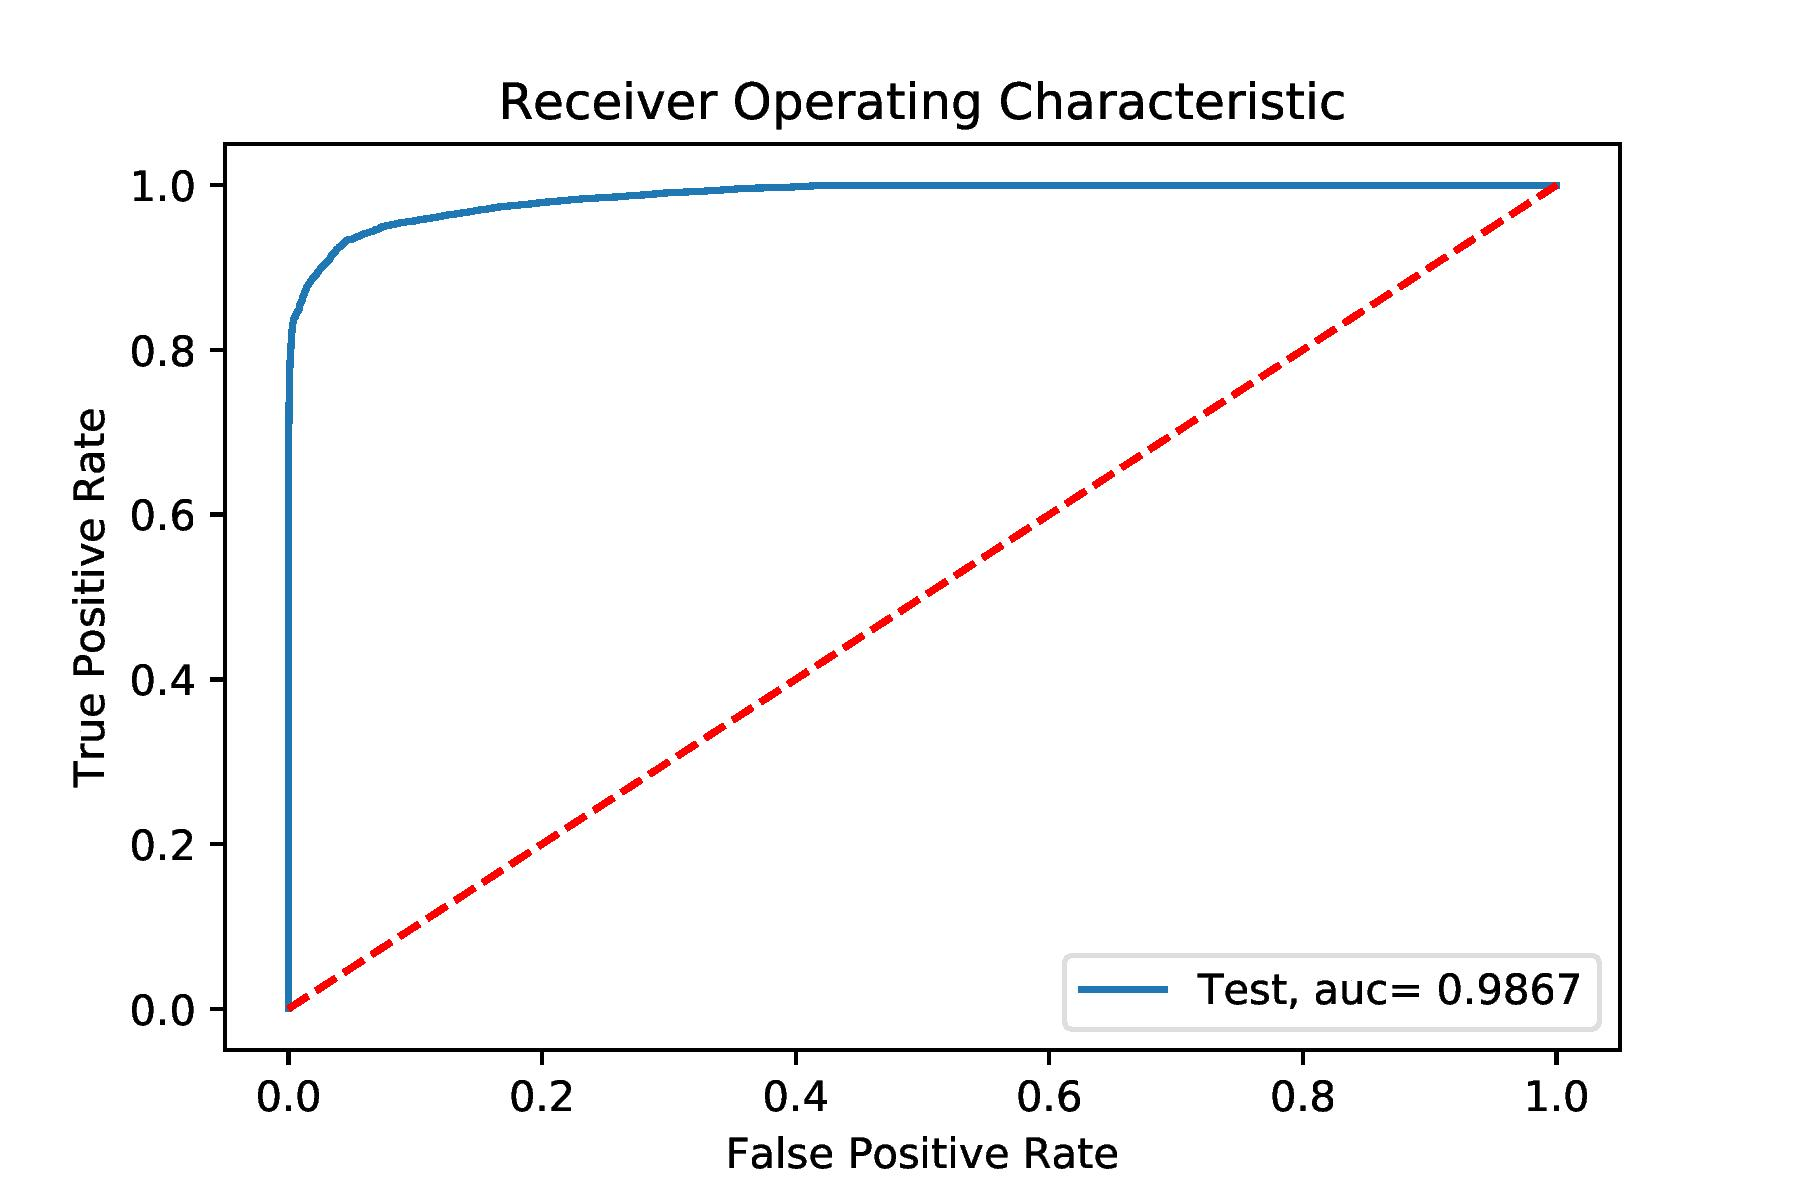
\includegraphics[width=\linewidth]{images/roc_test.jpg}
  \caption{ROC-AUC curve for validation on test data}
\label{fig:test}
\end{figure}


\section{Comparison with state-of-the-art models} \label{comparison}
In this section, we have compared our model performance with prior state-of-the-art models on the same dataset. We have arranged this section into subsections based on different experimentation setups that were followed in those works.



\subsection{Evaluation on train data}
Mogal et al. \cite{mogal2017nids} achieved 99.96\% accuracy on the UNSW-NB15 dataset using Naive Bayes and Logistic Regression,
which did not follow any cross-validation approach. A similar approach was taken by Kanimozhi et al. \cite{Kanimozhi2019UNSW-NB15} with the best four features chosen using the RandomForest classifier. The model achieved 98.3\% accuracy. We have shown in Table \ref{evaluationOnTrainData} that in the same validation process, our model has achieved near-perfect scores on both train and test data. We also did not find any comparison to
prior state-of-the-art with a similar validation process by Mogal et al. \cite{mogal2017nids} from Kanimozhi et al. \cite{Kanimozhi2019UNSW-NB15}.


\subsection{Ten-fold cross validation}
Suleiman et al.\cite{suleiman2018performance} evaluated performance using ten-fold cross-validation on train data. They found the Random Forest classifier to have the best accuracy and f1\_score. We have mentioned our model performance
using the same validation process in the train column of Table \ref{tenFoldCrossValidation}. TPR and recall are the same. Hence, we have mentioned only recall.


\begin{table}
\normalsize
\centering
\caption{Performance comparison with \cite{suleiman2018performance}}
\label{performanceComparisonWithSuleiman}
\renewcommand{\arraystretch}{1.2}
\begin{tabular}{|C{2.3cm}|C{2.2cm}|C{2.2cm}|}
\hline
\textbf{Metrics(\%)} & \textbf{RF \cite{suleiman2018performance}} & \textbf{LightGBM} \\ \hline
Accuracy & 90.14 & 96.17\\ \hline
Precision  & 99.8 & 96.54\\ \hline
Recall  & 97.8 & 97.89\\ \hline
F1\_score  & 98.7 & 97.20\\ \hline
FPR  & 0.1 & 7.48\\ \hline
\end{tabular}
\end{table}

Meftah et al. \cite{meftah2019network} applied ten-fold cross-validation on the train dataset and achieved the best accuracy 82.11\% using the SVM classifier. In the same validation process, our model accuracy is 96.17\%. Hanif et al. \cite{hanif2019intrusion} applied ten-fold cross-validation on the train and test dataset repeatedly using Artificial Neural Network(ANN) and achieved an average 84\% accuracy, 8\% false-positive rate. In a similar case, our model performance is better, 96.18\% accuracy and 7.47\% FPR as shown in Table \ref{tenFoldCrossValidation}. Though Meftah et al. \cite{meftah2019network} and Hanif et al. \cite{hanif2019intrusion} followed the same experimentation setup similar to Suleiman et al. \cite{suleiman2018performance}, none of them presented any comparison with it.

Koroniotis et al. \cite{koroniotis2017towards} performed ten-fold cross-validation on the combined dataset. The best result was achieved using the Decision Tree C4.5. In Table \ref{performanceComparisonWithKoroniotis} we have shown the comparison. Koroniotis et al. \cite{koroniotis2017towards} presented model performance with two metrics only, accuracy and FAR (False Alarm Rate). Our model has shown better performance in both of them.

\begin{table}
\normalsize
\centering
\caption{Comparison of our model with Koroniotis et al. \cite{koroniotis2017towards}}
\label{performanceComparisonWithKoroniotis}
\renewcommand{\arraystretch}{1.2}

\begin{tabular}{|C{3.3cm}|C{2.2cm}|C{1.5cm}|}
\hline
\textbf{Classifier} & \textbf{Accuracy (\%)} & \textbf{FAR(\%)} \\ \hline
Decision Tree \cite{koroniotis2017towards} & 93.23 & 6.77 \\ \hline
LightGBM & 95.19 & 4.81 \\ \hline
\end{tabular}
\end{table}

Nawir et al. \cite{nawir2019effective} applied a similar ten-fold cross-validation evaluation on the combined (train + test) dataset, using the WEKA J48 classifier. They have mentioned achieving high accuracy of 98.71\% using the default parameter. However, using exactly the same environment for multiple runs we have found that is not true.  It achieves around 94.6\% accuracy on average. That is lower than ours (95.19\%  accuracy).

\subsection{Five-fold cross validation}
We have found only Meghdouri et al. \cite{meghdouri2018analysis} to validate using five-fold cross-validation. Also, they have not mentioned any specific reason to avoid using ten-fold cross-validation, on which several works were already available at that moment. No performance comparison was also presented. Here we have not added any separate section for this. We have presented our model performance using same validation process in Table \ref{performanceComparisonWithMeghdouriTrain} and \ref{performanceComparisonWithMeghdouriTest}. Table \ref{performanceComparisonWithMeghdouriTrain} shows our model performance compared to theirs on five-fold cross-validation of the train dataset. Their model achieved higher accuracy (99\%) compared to ours (96.18\%). However, for precision, recall, and
f1\_score our model performance is much higher. Using the same validation process on the test dataset, from
Table \ref{performanceComparisonWithMeghdouriTest}, our test accuracy is very close to theirs.
However, like before our precision, recall and f1\_score are much better than theirs. Our ROC-AUC scores are very close too. For intrusion detection techniques f1\_score is very important, in which our model outperforms them by a large margin. 

% We have shown our ROC-AUC curve for this experiment in Figure \ref{fig:fiveFold}.

\begin{table}
\normalsize
\centering
\caption{Comparison with Meghdouri et al.\cite{meghdouri2018analysis} (Train data)}
\label{performanceComparisonWithMeghdouriTrain}
\renewcommand{\arraystretch}{1.2}
\begin{tabular}{|C{3cm}|C{2cm}|C{2cm}|}
\hline
\textbf{Metrics(\%)} & \textbf{Train\cite{meghdouri2018analysis}} & \textbf{Train} \\ \hline
Accuracy & 99.0 & 96.18\\ \hline
Precision  & 85.9 & 96.56 \\ \hline
Recall  & 85.1 & 97.87 \\ \hline
F1\_score  & 84.9 & 97.21 \\ \hline
ROC AUC  & 99.8 & 99.43 \\ \hline
\end{tabular}
\end{table}

\begin{table}
\normalsize
\centering
\caption{Comparison with Meghdouri et al.\cite{meghdouri2018analysis} (Test data)}
\label{performanceComparisonWithMeghdouriTest}
\renewcommand{\arraystretch}{1.2}
\begin{tabular}{|C{3cm}|C{2cm}|C{2cm}|}
\hline
\textbf{Metrics(\%)} & \textbf{Test\cite{meghdouri2018analysis}} & \textbf{Test} \\ \hline
Accuracy & 98.9 & 98.08\\ \hline
Precision  & 84.9 &  98.79\\ \hline
Recall & 85.1 & 97.7\\ \hline
F1\_score & 84.9 & 98.24 \\ \hline
ROC AUC   & 99.8& 99.81\\ \hline
\end{tabular}
\end{table}

% \begin{figure}[!tbh]
% \centering
%   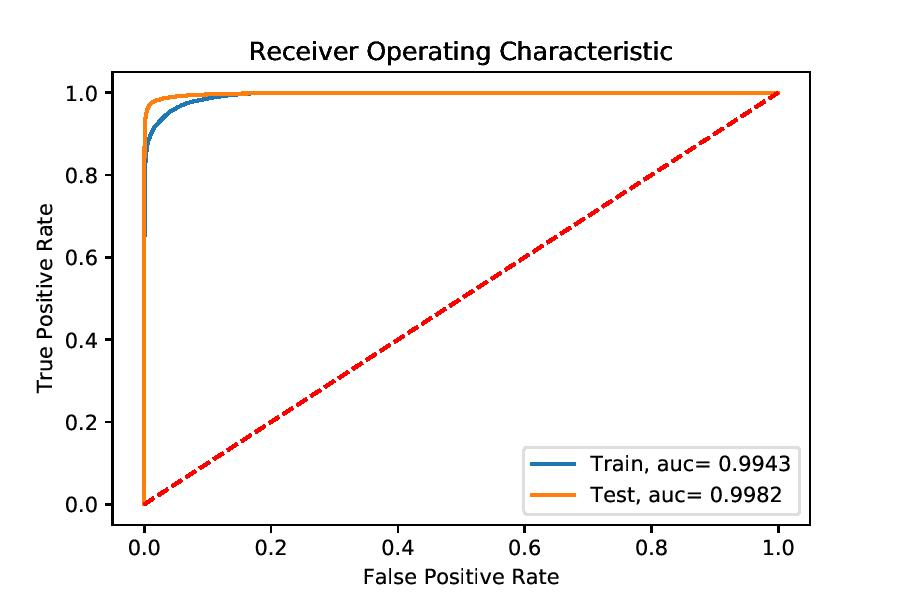
\includegraphics[width=\linewidth]{images/roc_five.jpg}
%   \caption{ROC-AUC curve for five-fold cross validation}
% \label{fig:fiveFold}
% \end{figure}

\subsection{Validation on separate test data}
Bhamare et al. \cite{bhamare2016feasibility} achieved accuracy 89.26\%, TP(True Positive) 93.7\% and TN (True Negative) 95.7\% at prediction threshold 0.5. Increasing the prediction threshold to 0.7-0.8 their TPR improved to 97\%, but TN dropped to 80\%. Where our accuracy, TP and TN are 91.95\%, 97\% and 86\% at threshold 0.5 as shown in Table \ref{confusionMatrix}. Moustafa et al. \cite{moustafa2016evaluation} achieved 85.56\% accuracy and 15.78\% FAR (False Alarm Rate) using DT (Decision Tree) technique built-in Visual Studio Business Intelligence 2008 with the default input parameters. Our model accuracy is 91.95\% and FAR 8.05\% FAR, which outperforms them in this validation setup.

\subsection{Others}
We have not been able to compare our results with some prior arts. For example Moustafa et al. \cite{moustafa2017hybrid} \cite{moustafa2018anomaly} \cite{moustafa2019holistic} evaluated the model on randomly chosen data from UNSW-NB15 dataset. However, it is not possible to reproduce the same random dataset. Also, we have not compared our model run time with prior arts as the run time environments are not the same.

% Belouch et al. \cite{belouch2018performance} found RandomForest classifier to achieve 97.49\% accuracy, 93.53\% sensitivity and 97.75\% specificity. However, it was not clear which validation approach was taken. 


\subsection{Results summary}

The followings are the summary of our results:
\begin{itemize}
    \item Validating on the same data used for training the model would give near-perfect results. However, it is due to overfitting. So this approach should not be followed.
    \item Feature engineering can make the model more generalized and improve performance on separate test data.
    \item There are many features having very low importance. Nearly 17 features have the importance of less than 1\%.
    \item Our model can better predict network anomaly than normal records. This is due to the presence of more anomalies in the dataset than normal.
\end{itemize}

\section{Conclusion \label{conclusion}}
In this paper, we have presented a boosting algorithm-based model for performing binary classification of the UNSW-NB15 dataset.
%We have explained all the steps taken from feature preprocessing, selection, and validation of the model. 
Different experimentation setups were followed to compare our performance with prior works. Results show that our model outperforms state-of-the-art works in most metrics. We have shown why the experimental setups followed by some prior works are heavily overfitted and should be avoided. Even when using a different cross-validation approach, our model outperforms most prior arts. Our model is also found to perform well on test data when it is fitted on train data only, validating the generalization of our model. So we believe this will help the network security community in improving anomaly detection. This study only performs a binary classification. However, our proposed algorithm can be easily adapted to multiclass-classification by changing LightGBM objective parameter to 'multiclass'. In the future, we intend to improve the performance of multiclass-classification on this dataset in a similar way.


\bibliography{bibliography}
\end{document}


